

La figure \ref{transformationimage} nous montre un exemple de transformation d'une image de maison réalisée en 2 traits de crayons. 

\begin{figure}[h]
	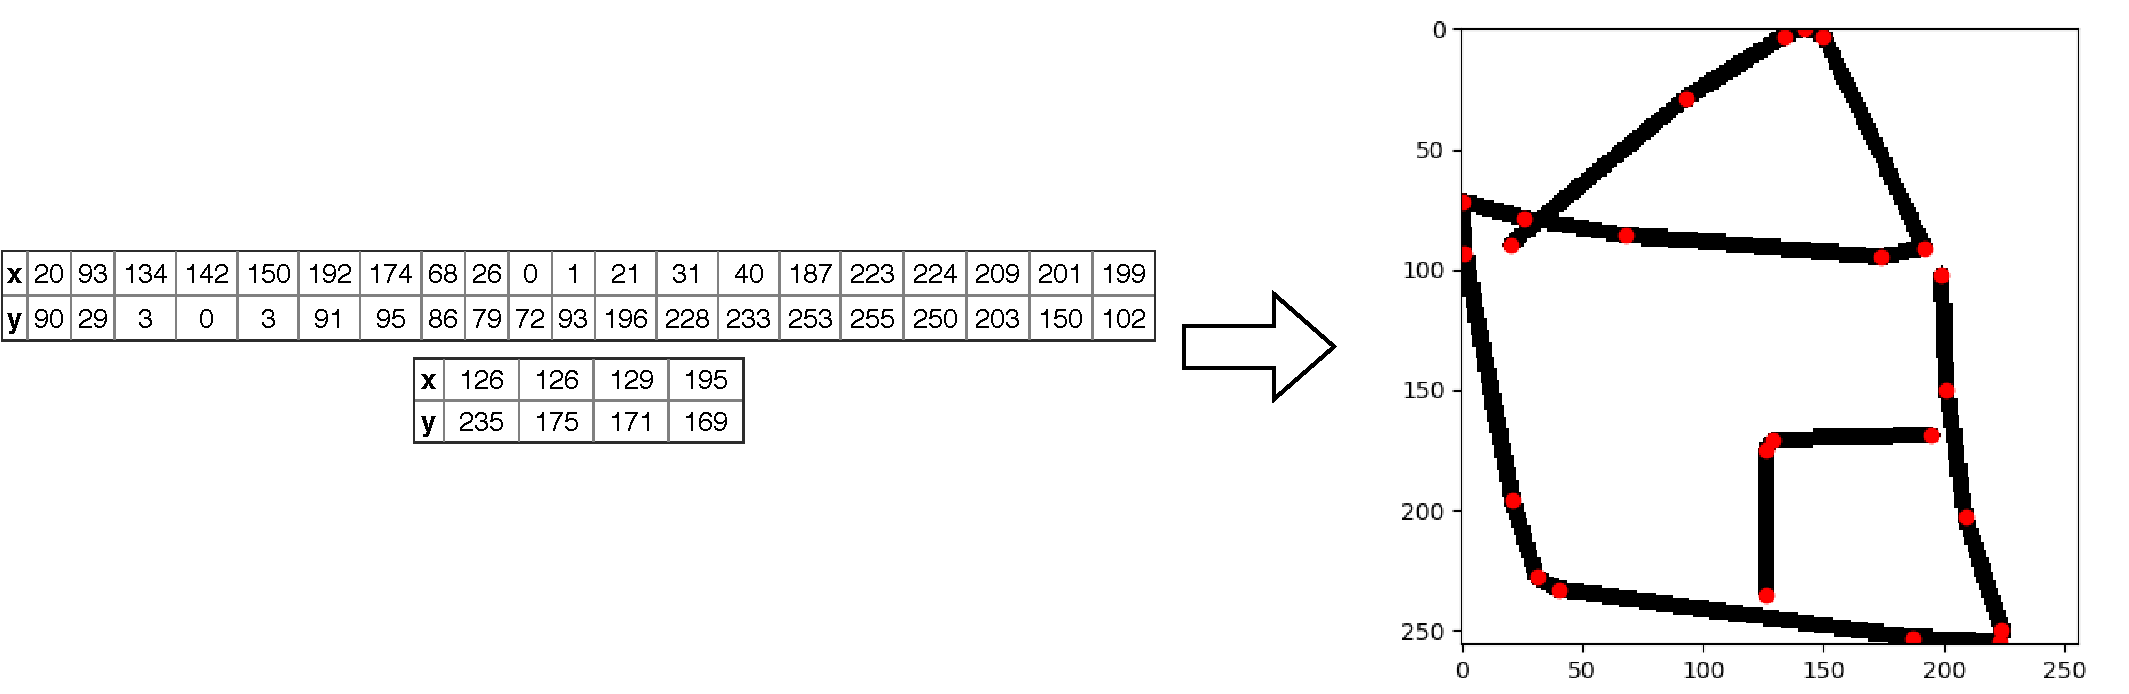
\includegraphics[width=\linewidth]{images/Transformations_horizontal.pdf} % Figure image
	\caption{Transformation de vecteur à image} % Figure caption
	\label{transformationimage} 
\end{figure}

On passe donc d'une série de positions en format vectoriel à une image 256x256 à un seul canal en noir et blanc lorsqu'on vient charger les données dans notre modèle. 
Cette technique nous évite de stocker toutes les données sous forme d'images qui doubleraient facilement la quantité de données à emmagasiner pour traitement. 


La plupart des images sont loin d'être faciles à apprendre pour un ordinateur, puisqu'il existe une multitude de façons de dessiner une même classe.
N'importe quel individu peut contribuer à cette base de données de dessins, ce qui fait en sorte qu'on a une grande variété de dessins différents pour une classe donnée. La figures \ref{frogs} nous permet de voir différentes images pour la classe \emph{frog}.


\begin{figure}[h]
	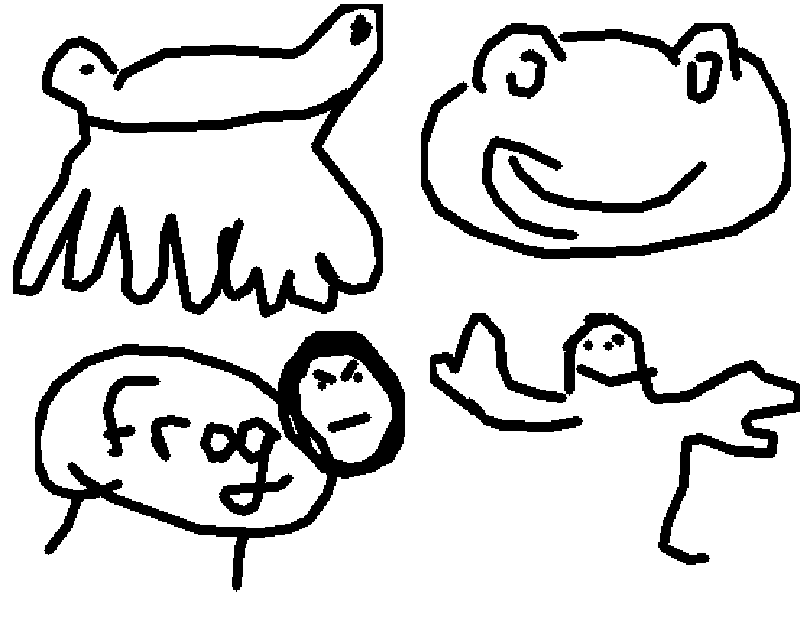
\includegraphics[width=\linewidth]{images/Combo_frogs.png} % Figure image
	\caption{Différentes images de la classe frog} % Figure caption
	\label{frogs} 
\end{figure}


On peut voir que les utilisateurs n'adoptent pas tous les mêmes formes pour dessiner un même objet. 
Également, puisque les utilisateurs ont seulement 20 secondes pour faire leur dessin, certains d'entre eux sont parfois incomplets.
Notre modèle doit donc apprendre à composer avec cette grande variabilité et faire une prédiction précise même lorsqu'un dessin est partiel.

